\documentclass[14pt]{beamer}

\usepackage[english]{babel}

\usepackage[latin1]{inputenc}

\usepackage[T1]{fontenc}

\usepackage{amsmath}
\usepackage{amsfonts}
\usepackage{amssymb}
\usepackage{amsthm}

%\usepackage{tgtermes}
\usepackage{tgheros}
%\usepackage{cmbright}
\usepackage{qtxmath}
%\usepackage{kpfonts}
\renewcommand{\ttdefault}{txtt}

%\usepackage[amsmath,thmmarks]{ntheorem}

\usepackage{graphics}
\usepackage{url}
\usepackage{listings}
\lstset{
  numbers=none,
  basicstyle=\footnotesize\ttfamily,
  xleftmargin=1em,
  xrightmargin=0em,
  aboveskip=1em,
  belowskip=1em
}

\usepackage{tikz}
\usetikzlibrary{shapes,snakes,positioning}

\tikzstyle{mybox} = [draw=red, fill=blue!20, very thick,
    rectangle, rounded corners, inner sep=10pt, inner ysep=12pt]
\tikzstyle{fancytitle} = [fill=red, text=white]

\setbeamertemplate{navigation symbols}{}
\setbeamertemplate{headline}{}
\setbeamertemplate{footline}{}
\usetheme{default}
%\usecolortheme[named=red]{structure}


\title{Software Licensing\\
  {\small the GPL in combination with closed source software}}

\author{Martijn Vermaat}
\institute{Human Genetics, LUMC}
\date{\small Bioinformatics work discussion, October 25, 2011}


\begin{document}


\frame{\titlepage}


\frame{

  \frametitle{Intellectual property (IP) law}

  \begin{itemize}
    \item creations of the mind
    \item for which property rights are recognized
    \item various fields of law
    \item exclusive rights
    \item in some jurisdictions
  \end{itemize}

}


\frame{

  \frametitle{IP rights}

  \begin{itemize}
    \item {\bf copyrights}
    \item {\bf patents}
    \item {\bf trade marks}
    \item database rights
    \item breeder rights
    \item portrait rights
    \item \ldots
  \end{itemize}

}


\frame{

  \frametitle{Copyright}

  \begin{itemize}
    \item free
    \item long-lasting
    \item international
    \item no formalities
  \end{itemize}

  works that are
  \begin{itemize}
    \item not copied
    \item the result of creative choices
  \end{itemize}

}


\frame{

  \frametitle{Works protected by copyright}

  every original work of authorship, irrespective of its literary or
  artistic merit. the ideas in the work do not need to be original,
  but the form of expression must be an original creation of the
  author.

  examples:
  \begin{itemize}
    \item {\bf books}
    \item maps
    \item sheet music
    \item dramatic works
    \item paintings
    \item photographs
    \item architectural drawings
    \item sound recordings
    \item motion pictures
    \item computer programs
  \end{itemize}

}


\frame{

  \frametitle{Rights protected by copyright}

  \begin{itemize}
    \item reproduction in various forms, such as printed publications or sound recordings
    \item distribution of copies
    \item public performance
    \item broadcasting or other communication to the public
    \item translation into other languages
    \item adaptation, such as a novel into a screenplay
  \end{itemize}

  duration: at least life of the author plus 50 years (but getting longer)

}


\frame{

  \frametitle{Licensing}

  give others some of your exclusive rights (under certain conditions)

}


\frame{

  \frametitle{Open Source}

  Permissive licenses

  Copyleft licenses

}


\frame{

  \frametitle{MIT license}

  Not public domain!

}


\frame{

  \frametitle{GNU General Public License}

  The GNU General Public License is a free, copyleft license for
  software and other kinds of works.

}


\frame{

  \frametitle{MySQLdb}

  Case study: using MySQL from a Python program

  \vspace{\baselineskip}

  \begin{itemize}
    \item MySQL (client and server) is GPL-licensed
    \item Python MySQLdb library is GPL-licensed
    \item MySQLdb uses libmysql (part of MySQL)
  \end{itemize}

}


\frame{

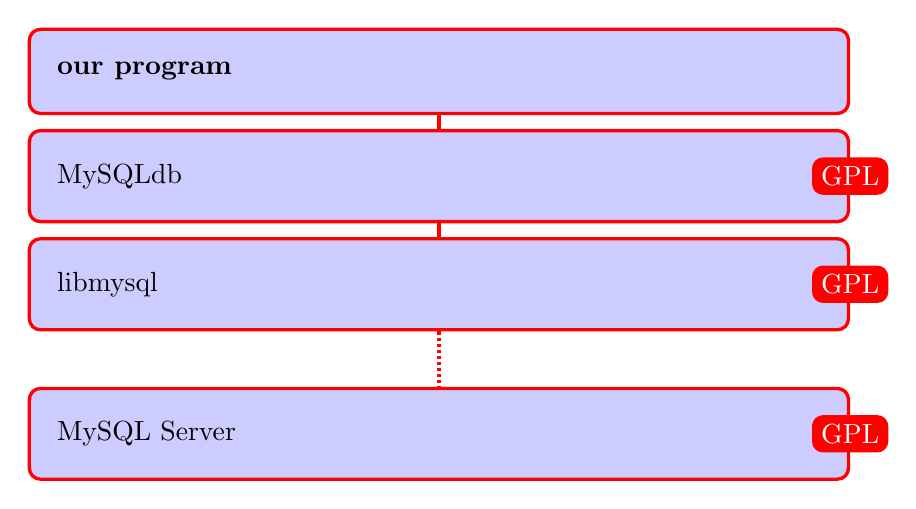
\begin{tikzpicture}

\node [mybox] (box1){%
    \begin{minipage}{0.80\linewidth}
      {\bf our program}
    \end{minipage}
};

\node [mybox,below=5pt of box1.south] (box2) {%
    \begin{minipage}[t!]{0.8\linewidth}
      MySQLdb
    \end{minipage}
    };
\node[fancytitle, rounded corners] at (box2.east) {GPL};

\draw [mybox] (box1) -- (box2);

\node [mybox,below=5pt of box2.south] (box3) {%
    \begin{minipage}[t!]{0.8\linewidth}
      libmysql
    \end{minipage}
    };
\node[fancytitle, rounded corners] at (box3.east) {GPL};

\draw [mybox] (box2) -- (box3);

\node [mybox,below=20pt of box3.south] (box4) {%
    \begin{minipage}[t!]{0.8\linewidth}
      MySQL Server
    \end{minipage}
    };
\node[fancytitle, rounded corners] at (box4.east) {GPL};

\draw[style=densely dotted] [mybox] (box3) -- (box4);

\end{tikzpicture}

}


\frame{

  \frametitle{MySQLdb license}

  Is it really GPL-licensed?

  \begin{itemize}
    \item Most Linux distributions say GPL
    \item Sourceforge project page says ``GNU General Public License
      (GPL), Python License (CNRI Python License), Zope Public License''
    \item Source code says ``GPL or the original license based on Python
      1.5.2's license''
  \end{itemize}

  The Python 1.5.2 license is an MIT-like license ({\em not} the CNRI
  Python License)

}


\frame{

  \frametitle{GPL violation?}

  MySQLdb links to libmysql (GPL)

  \vspace{\baselineskip}

  Doesn't MySQLdb's dual licensing violate libmysql's GPL
  license?

}


\frame{

  \frametitle{libmysql}

  MySQL FLOSS License Exception:
  \begin{quote}We want specified Free/Libre and Open Source Software (``FLOSS'')
    applications to be able to use specified GPL-licensed MySQL client
    libraries (the ``Program'') despite the fact that not all FLOSS
    licenses are compatible with version 2 of the GNU General Public
    License (the ``GPL'').
  \end{quote}

}


\frame{

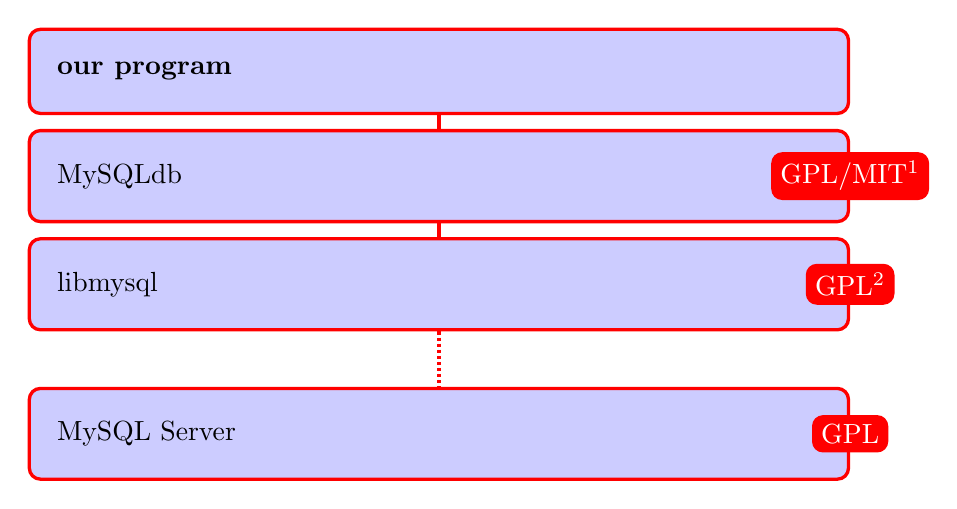
\begin{tikzpicture}

\node [mybox] (box1){%
    \begin{minipage}{0.80\linewidth}
      {\bf our program}
    \end{minipage}
};

\node [mybox,below=5pt of box1.south] (box2) {%
    \begin{minipage}[t!]{0.8\linewidth}
      MySQLdb
    \end{minipage}
    };
\node[fancytitle, rounded corners] at (box2.east) {GPL/MIT$^1$};

\draw [mybox] (box1) -- (box2);

\node [mybox,below=5pt of box2.south] (box3) {%
    \begin{minipage}[t!]{0.8\linewidth}
      libmysql
    \end{minipage}
    };
\node[fancytitle, rounded corners] at (box3.east) {GPL$^2$};

\draw [mybox] (box2) -- (box3);

\node [mybox,below=20pt of box3.south] (box4) {%
    \begin{minipage}[t!]{0.8\linewidth}
      MySQL Server
    \end{minipage}
    };
\node[fancytitle, rounded corners] at (box4.east) {GPL};

\draw[style=densely dotted] [mybox] (box3) -- (box4);

\end{tikzpicture}

\vspace{\baselineskip}

$^1$ dual-licensed\\
$^2$ with client exception

}


\frame{

  \frametitle{Acknowledgements}

  Software Licensing Workshop\\
  {\small NBIC, September 8, 2011}

  \vspace{\baselineskip}

  Maurits Westerik\\
  {\small Bird\&Bird}

  \vspace{\baselineskip}

  Peter Taschner\\
  Ivo Fokkema\\
  Jeroen Laros\\
  {\small Human Genetics, LUMC}

}


\end{document}
